\documentclass[10pt]{article}
\usepackage{amsmath}
\usepackage{amssymb}
\usepackage{graphicx}
\usepackage[left=2cm,right=2cm,top=2cm,bottom=2cm,a4paper]{geometry}
\title{Numerical Analysis\\ Homework \#1}
\author{Junyoung, Jang (2013314051)}
\date{\today}
\begin{document}
\maketitle
	\begin{flushleft}
 	\textbf{1.} Find the roots of the following equations by using Bisection, Newton's and Secant methods.\\
 	\quad\,Comapare the convergence(verify with real numbers).\\
 	\quad\,\textbf{(1)} $e^x -3x^2=0$\\
 	\;
 	\qquad \quad \textbf{(Solution.)} \\
	\qquad \quad We can find roots using Rootfinding Method. I choose error boundary less than $\epsilon$\\ 
	\qquad \quad First, We find intersection point of $e^x$ and $3x^2$ or using $f(x)f(y)<0$\\
	\begin{figure}[!h]
		\centering
		\begin{center}
		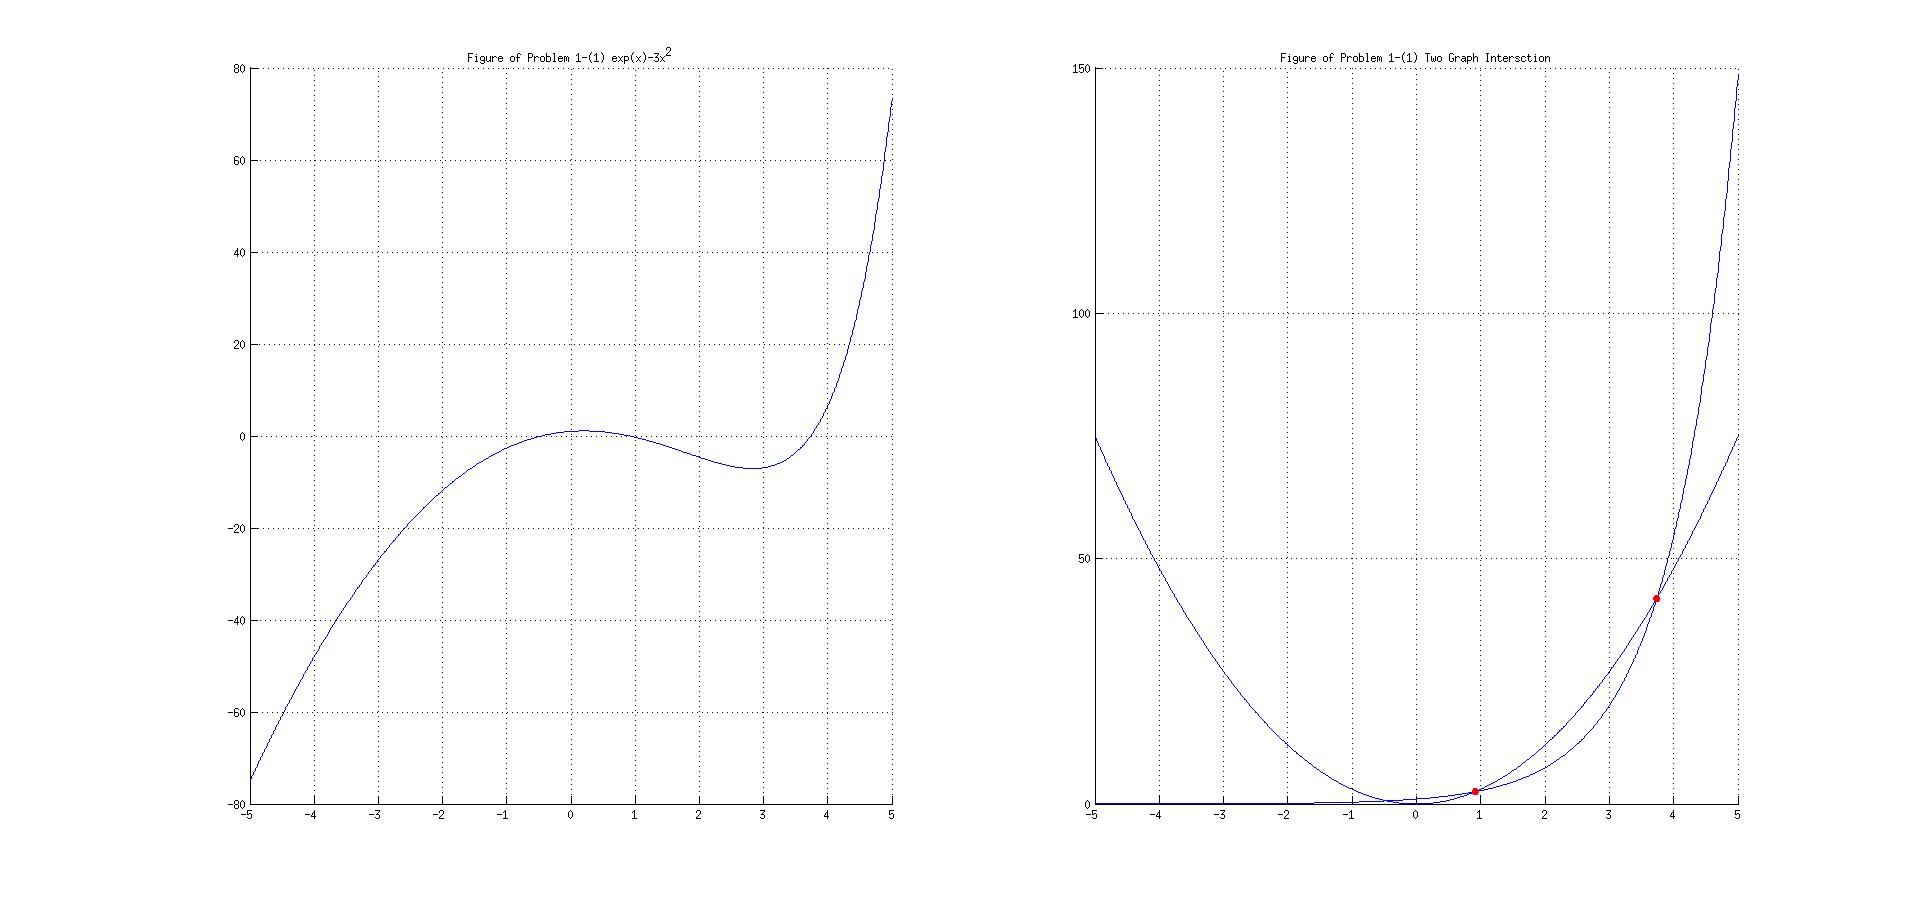
\includegraphics[width=0.8\textwidth]{1-1.png}
		\caption{Problem 1-(1), Graph.}
		\end{center}
	\end{figure}
	\qquad \quad Redpoint of Right Graph of Figure 1. is Roots. Problem 1-(1) have two roots.\\
	\qquad \quad Therefore, Using rootfinding method,\\
	\begin{figure}[!h]
		\centering
		\begin{center}
		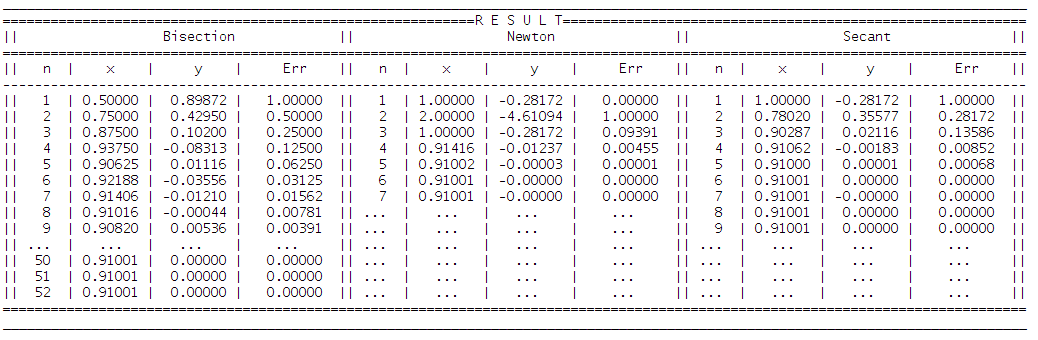
\includegraphics[width=0.9\textwidth]{1-1-r1.png}
		\caption{Problem 1-(1), Result of 1 near root }
		\end{center}
	\end{figure}
	\qquad \quad We choose initial condition,\\
	\qquad \qquad \qquad \qquad \qquad \textbf{Bisection: $x_0=0,x_1=1$, Newton: $x_0=1$, Secant: $x_0=0,x_1=1$}\\
	\qquad \quad We aleady know this result. Because we learned convergence speed. We have result as expected.\\
	\qquad \quad Therefore, We know convergence speed which is Bisection $<<$ Secant $ < $ Newton.\\
	\qquad \quad Next, We once more find root which is near 3. Similary, using rootfinding method,\\*
	\begin{figure}[!h]
		\centering
		\begin{center}
		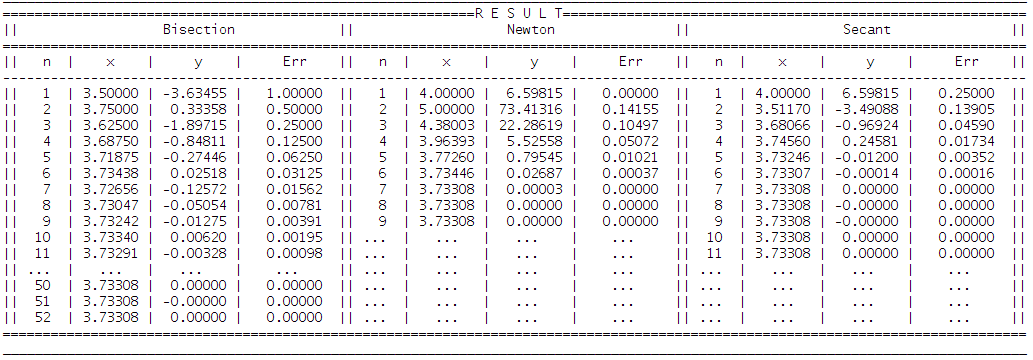
\includegraphics[width=0.9\textwidth]{1-1-r2.png}
		\caption{Problem 1-(1), Result of 3 near root }
		\end{center}
	\end{figure}
	\qquad \quad We can know convergence speed, as known above. Therefore, we can check that i learned in theory.\\
	\;
	\quad\,\textbf{(2)} $x^3=x^2+x+1$\\
	\;\;\;
	\qquad \quad \textbf{(Solution.)} \\
	\qquad \quad Similary, we can find roots using Rootfinding Method. I choose error boundary less than $\epsilon$\\ 
	\qquad \quad First, We find intersection point of $x^3$ and $x^2+x+1$ or using $f(x)f(y)<0$\\
	\begin{figure}[!h]
		\centering
		\begin{center}
		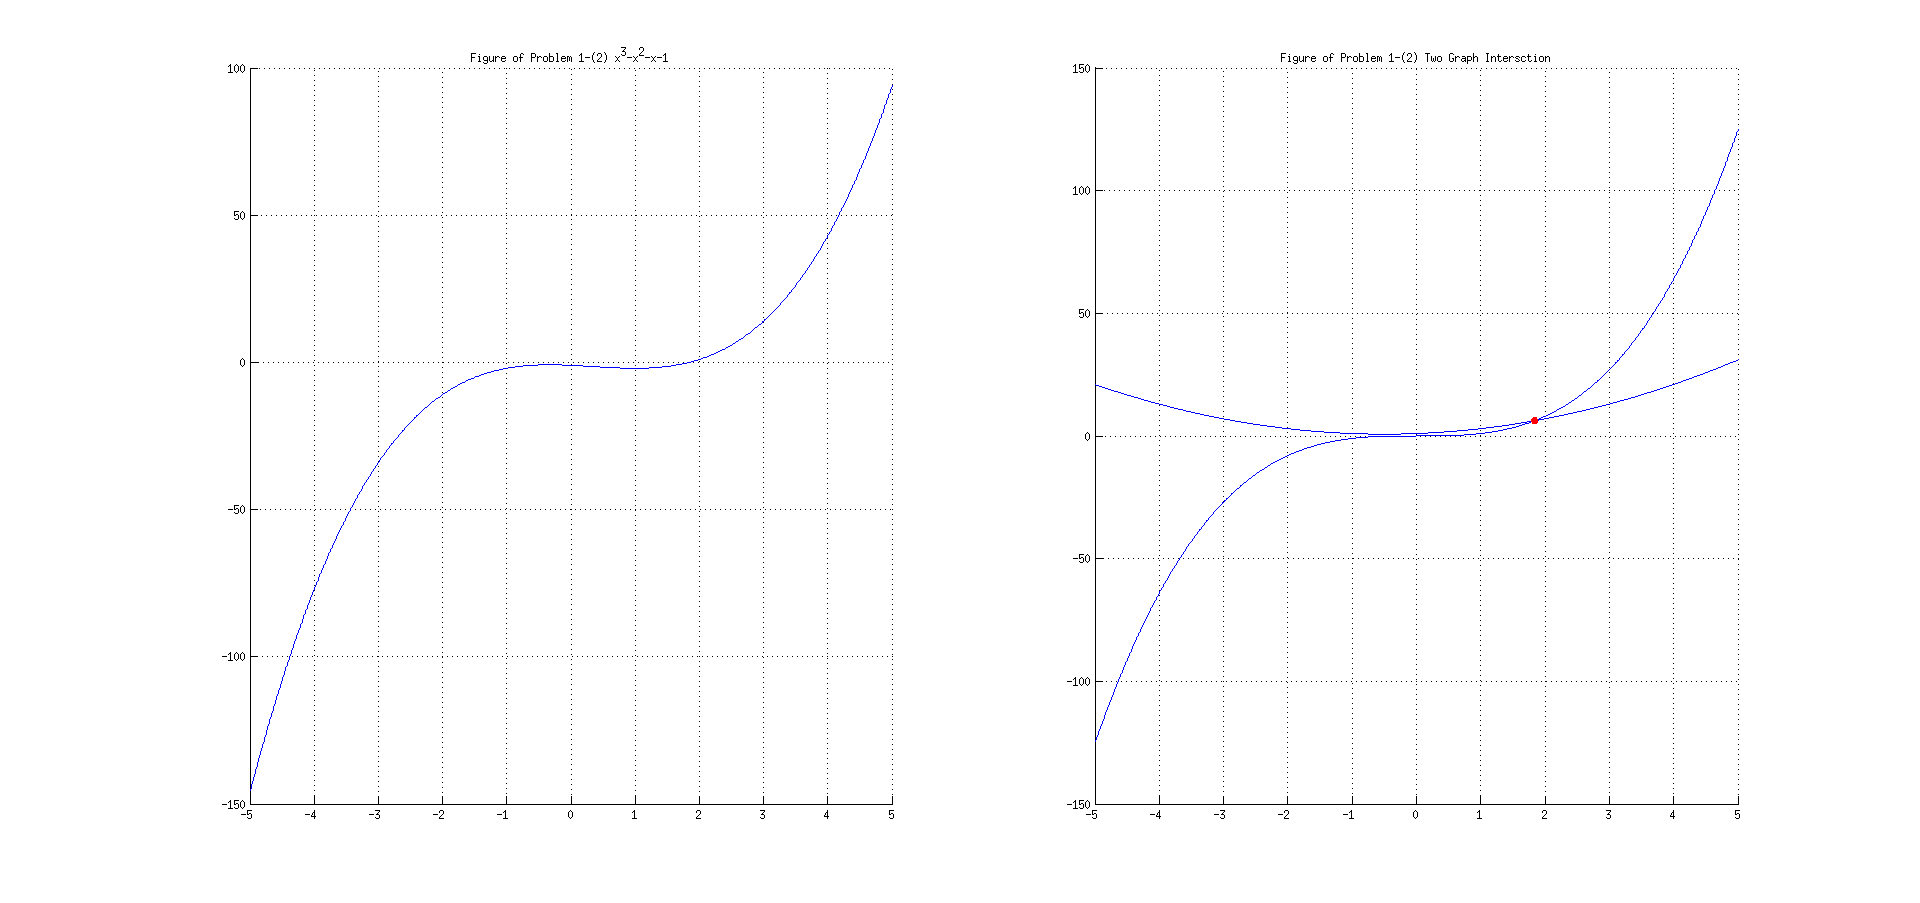
\includegraphics[width=0.8\textwidth]{1-1-2.png}
		\caption{Problem 1-(2), Graph.}
		\end{center}
	\end{figure}
	\qquad \quad Problem 1-(2) have one root near 2.Therefore, Using rootfinding method,\\
	\begin{figure}[!h]
		\centering
		\begin{center}
		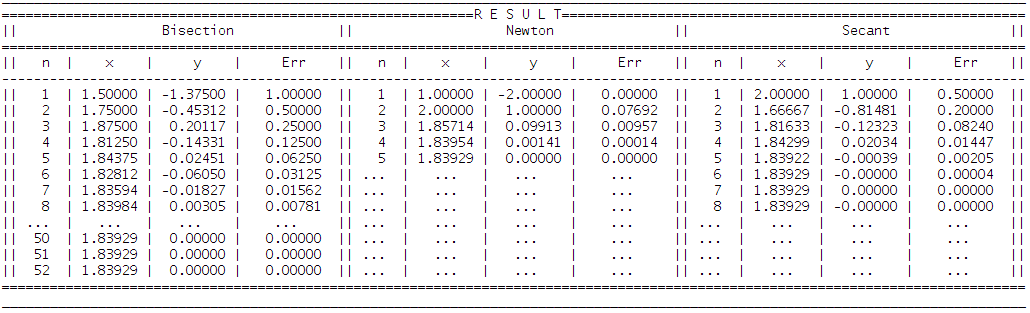
\includegraphics[width=0.9\textwidth]{1-2-r.png}
		\caption{Problem 1-(2), Result of 2 near root }
		\end{center}
	\end{figure}
	\qquad \quad We choose initial condition,\\
	\qquad \qquad \qquad \qquad \qquad \textbf{Bisection: $x_0=1,x_1=2$, Newton: $x_0=1$, Secant: $x_0=1,x_1=2$}\\
	\qquad \quad Like Problem (1), We have similar result. We can know centain comparison of convergence speed. \\
	\qquad \qquad \qquad \qquad \qquad\qquad\qquad\qquad\qquad   Bisection $<<$ Secant $ < $ Newton.\\
	\;\;\;\;
	\quad\,\textbf{(3)} $e^x=\frac{1}{0.1+x^2}$\\
	\;\;\;
	\qquad \quad \textbf{(Solution.)} \\
	\qquad \quad Similary, we can find roots using Rootfinding Method. I choose error boundary less than $\epsilon$\\ 
	\qquad \quad First, We find intersection point of $e^x$ and $\frac{1}{0.1+x^2}$ or using $f(x)f(y)<0$\\
	\begin{figure}[!h]
		\centering
		\begin{center}
		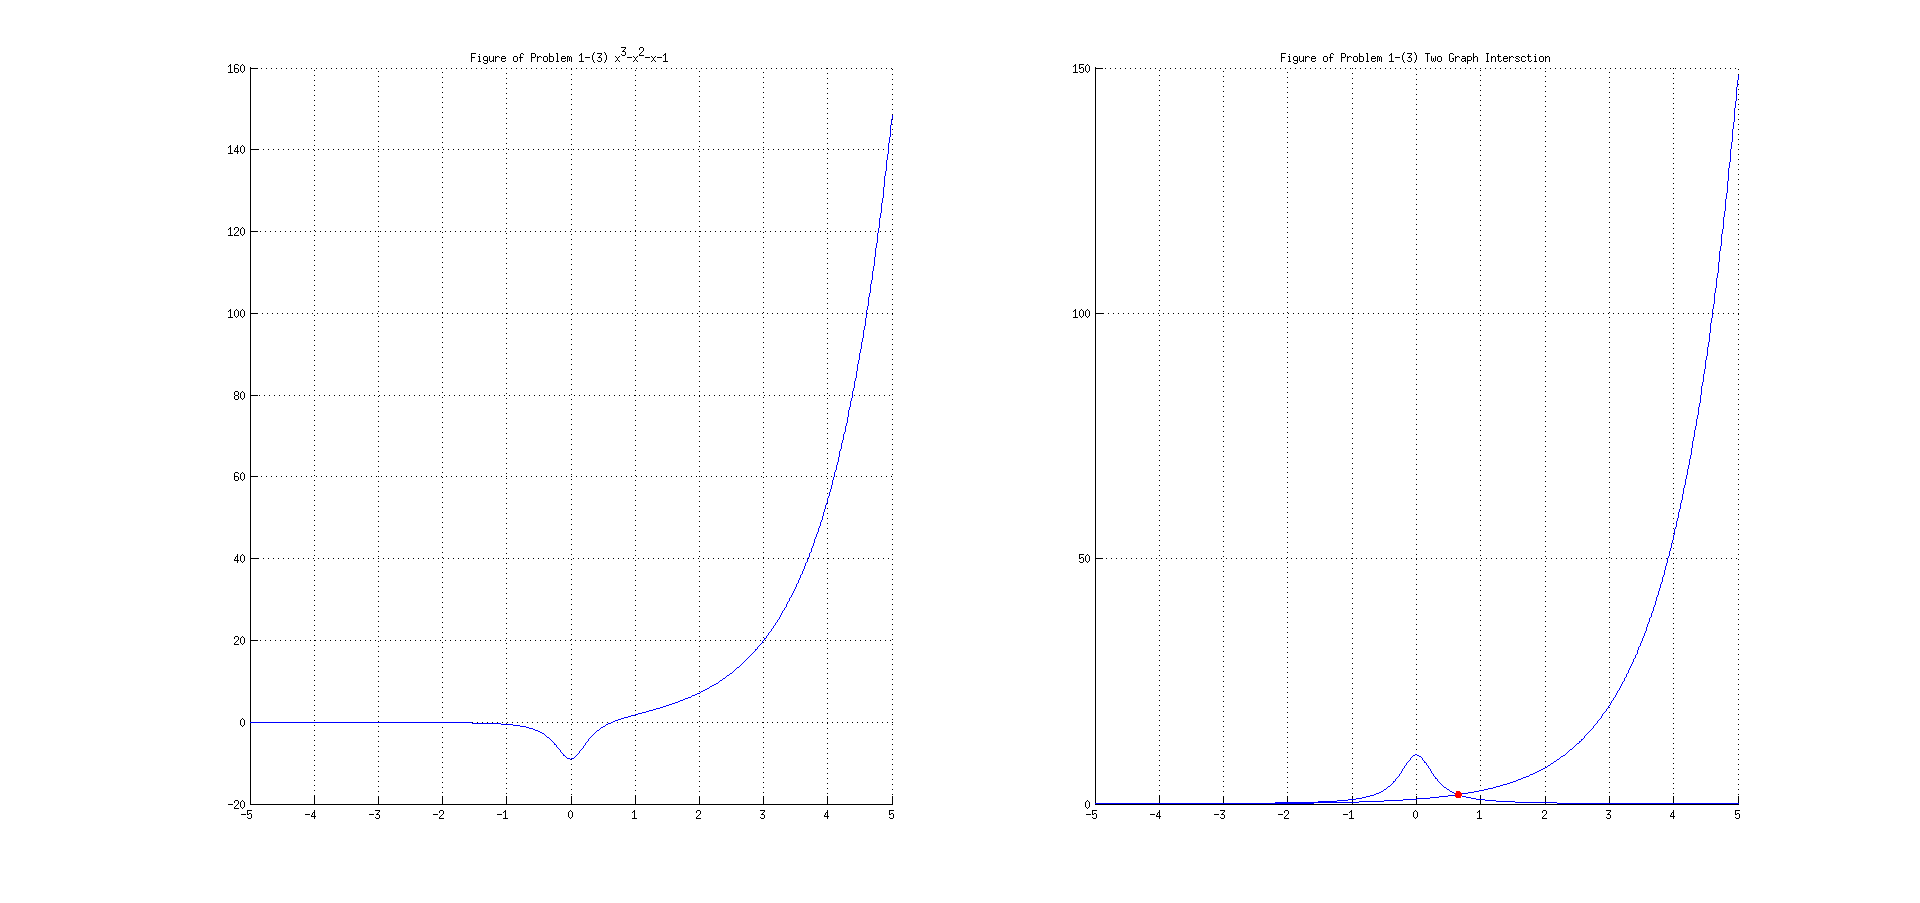
\includegraphics[width=0.8\textwidth]{1-1-3.png}
		\caption{Problem 1-(3), Graph.}
		\end{center}
	\end{figure}
	\qquad \quad Problem 1-(3) have one root near 1.Therefore, Using rootfinding method,\\
	\begin{figure}[!h]
		\centering
		\begin{center}
		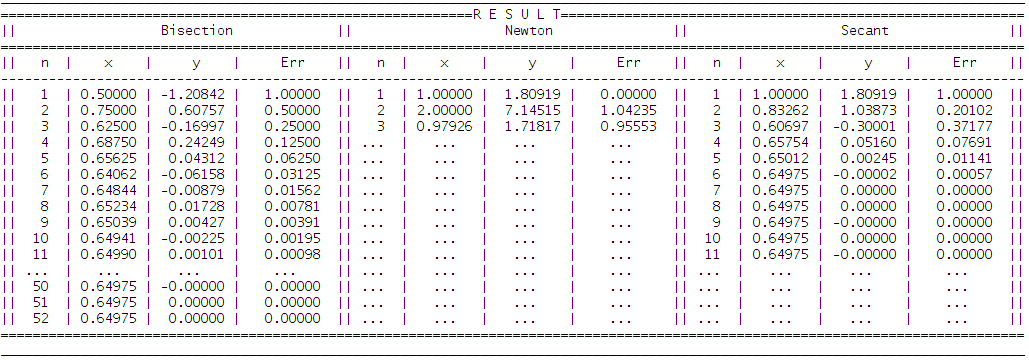
\includegraphics[width=0.9\textwidth]{1-3-r.png}
		\caption{Problem 1-(3), Result of 1 near root }
		\end{center}
	\end{figure}
	\qquad \quad We choose initial condition,\\
	\qquad \qquad \qquad \qquad \qquad \textbf{Bisection: $x_0=0,x_1=1$, Newton: $x_0=1$, Secant: $x_0=0,x_1=1$}\\
	\qquad \quad We can get different result from above. Newton Method don't have convergence point.\\
	\qquad \quad Since there is not differential value of $f(x)=e^x-\frac{1}{0.1+x^2}$ at x=0 and $f'=0$ where $x<-1$.Therefore, \\
	\qquad \quad no longer newton method don't work. We can know disadvantage of Newton method above result.\\
 	\;\;\;\;\newpage
 	\quad\,\textbf{(4)} $x=1+0.3\cos(x)$\\
 	\;\;\;
	\qquad \quad \textbf{(Solution.)} \\
	\qquad \quad Similary, we can find roots using Rootfinding Method. I choose error boundary less than $\epsilon$\\ 
	\qquad \quad First, We find intersection point of $x$ and $1+0.3\cos(x)$ or using $f(x)f(y)<0$\\
	\begin{figure}[!h]
		\centering
		\begin{center}
		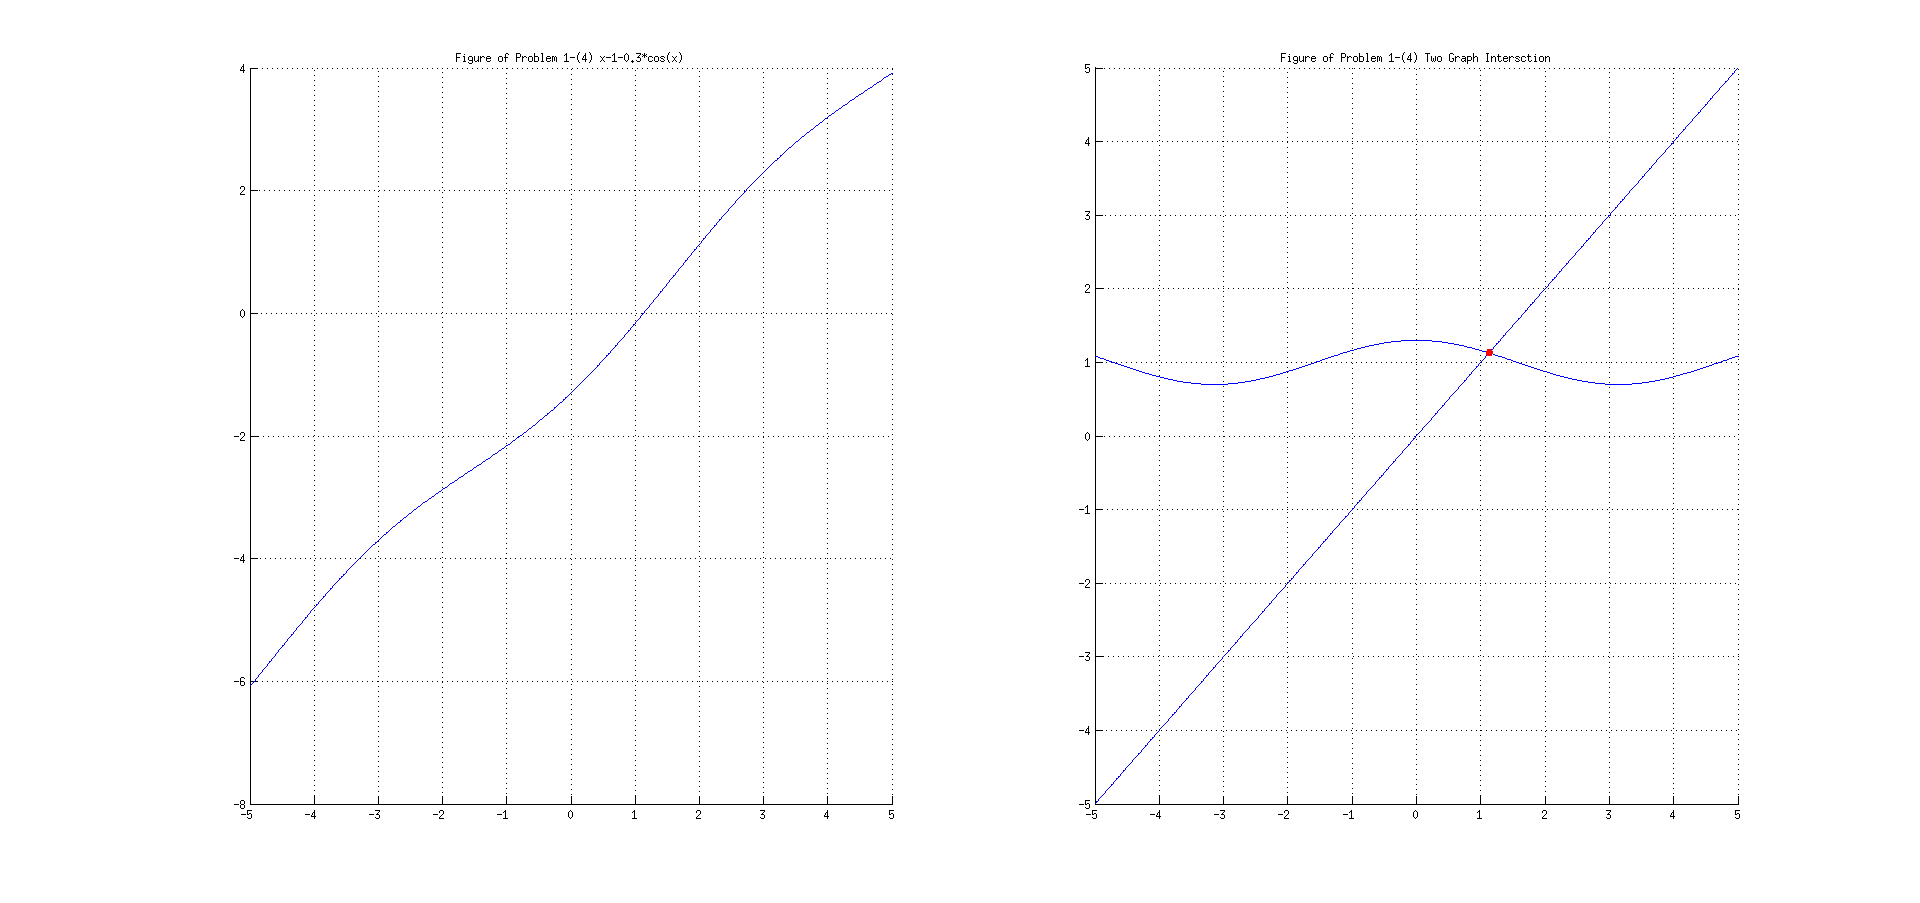
\includegraphics[width=0.8\textwidth]{1-1-4.png}
		\caption{Problem 1-(4), Graph.}
		\end{center}
	\end{figure}
	\qquad \quad Problem 1-(4) have one root near 1.Therefore, Using rootfinding method,\\
	\begin{figure}[!h]
		\centering
		\begin{center}
		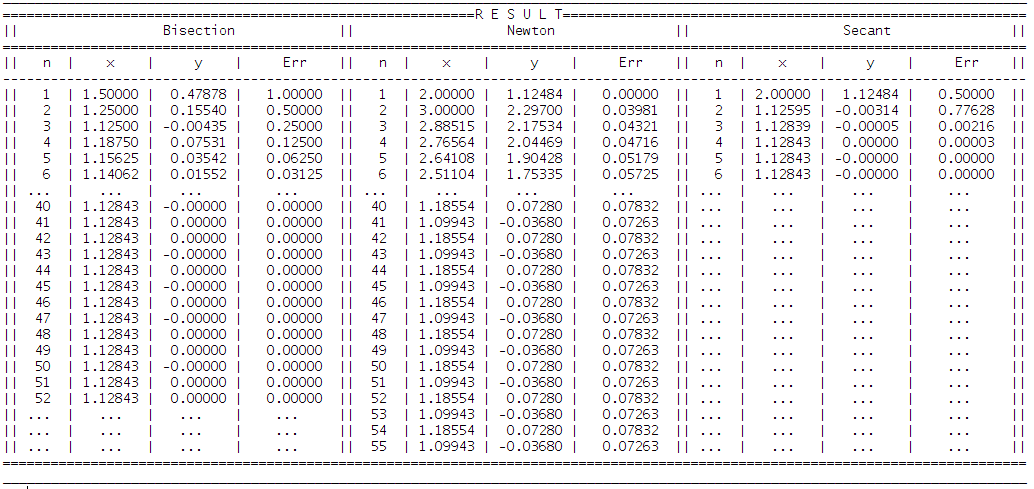
\includegraphics[width=0.9\textwidth]{1-4-r.png}
		\caption{Problem 1-(4), Result of 1 near root }
		\end{center}
	\end{figure}
	\qquad \quad We choose initial condition,\\
	\qquad \qquad \qquad \qquad \qquad \textbf{Bisection: $x_0=1,x_1=2$, Newton: $x_0=2$, Secant: $x_0=1,x_1=2$}\\
	\qquad \quad We can know disadvantage of Newton Method. This situation is Cycling of Newton Method.\\
	\qquad \quad Newton Method don't convergence a point.\\
	\;\;\;
	\qquad \quad \textbf{- Comment}\\
	\qquad \qquad Newton Method have the fastest convergence speed. But we should careful use it.\\
	\qquad \qquad Since (3) and (4) situation are able to occur. Because We can know Newton Method always don't\\
	\qquad \qquad haveguarantee to find root. Maybe, I think Newton Method use diffential value. On the other hand, \\
	\qquad \qquad Bisection and Secant Method converge well.\\
	\qquad \qquad(Bisection and Secant Method are covergence speed less than Newton method.)\\
	\qquad \qquad I think most important choose initial condition and looking to characteristics of the function.\\
	\;\;\;\;\;\;\newpage
	\textbf{2.} Witch of the following iterations will converge to the indicated fixed point $\alpha$ (provided $x_0$ is sufficiently\\
	\quad\, close to $\alpha$)? If it does converge, give the order of convergence; for linear convergence, give the rate of linear \\
	\quad\, convergence.\\
	\quad\,\textbf{(a)} $x_{n+1}=-16+6x_n+12/x_n,\quad \alpha=2$\\
	\;\;\;
	\qquad \quad \textbf{(Solution.)} \\
	\qquad \quad Before using Fixed Point Method, Looking at Graph of $f(x)=-16+6x+12/x$\\
	\begin{figure}[!h]
		\centering
		\begin{center}
		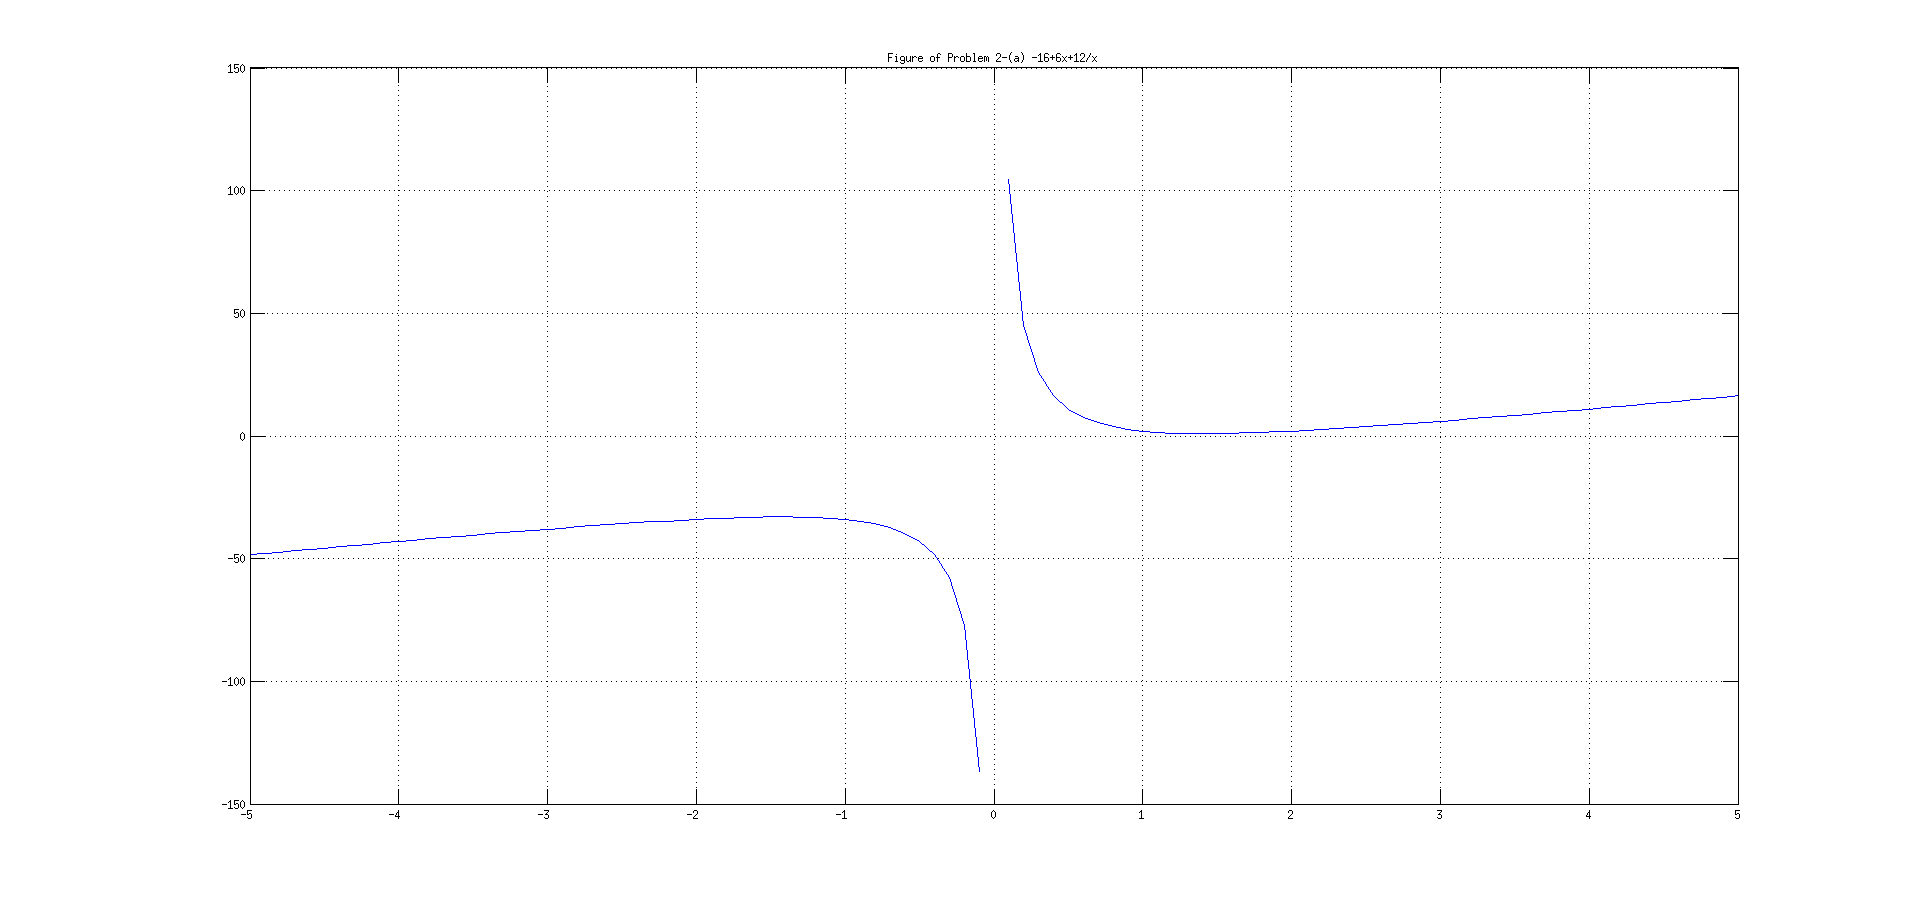
\includegraphics[width=1\textwidth]{2-a.png}
		\caption{Problem 2-(a), $-16+6x+12/x$ }
		\end{center}
	\end{figure}
	\qquad \quad We can know $f(x)$ don't have root. Using Fixed Point Method, \\
	\begin{figure}[!h]
		\centering
		\begin{center}
		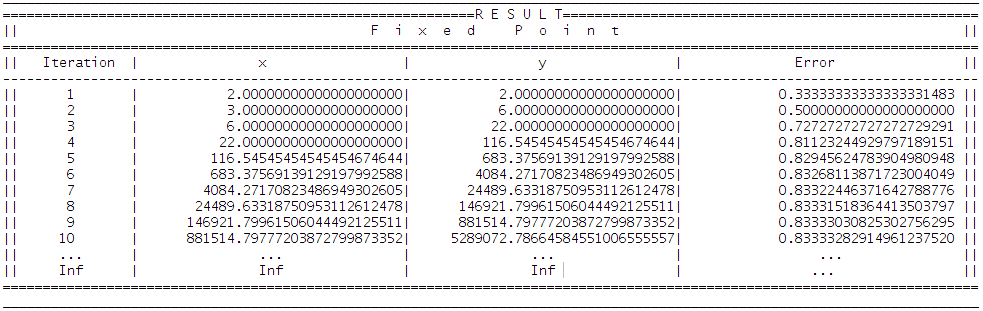
\includegraphics[width=0.9\textwidth]{2-ra.png}
		\caption{Problem 2-(a), Result}
		\end{center}
	\end{figure}
	\qquad \quad We choose initial condition. $x_0=2+\epsilon$ and relative error boundary less than $\epsilon$.\\
	\qquad \quad Therefore, We can know this function is divergence using fixed point method.\\
	\;\;\;\;\newpage
	\quad\,\textbf{(b)} $x_{n+1}=-2x_n/3+1/x_n^2,\quad \alpha=3^{\frac{1}{3}}$\\
	\;\;\;
	\qquad \quad \textbf{(Solution.)} \\
	\qquad \quad Similary, Before using Fixed Point Method, Looking at Graph of $f(x)=-2x/3+1/x^2$\\
	\begin{figure}[!h]
		\centering
		\begin{center}
		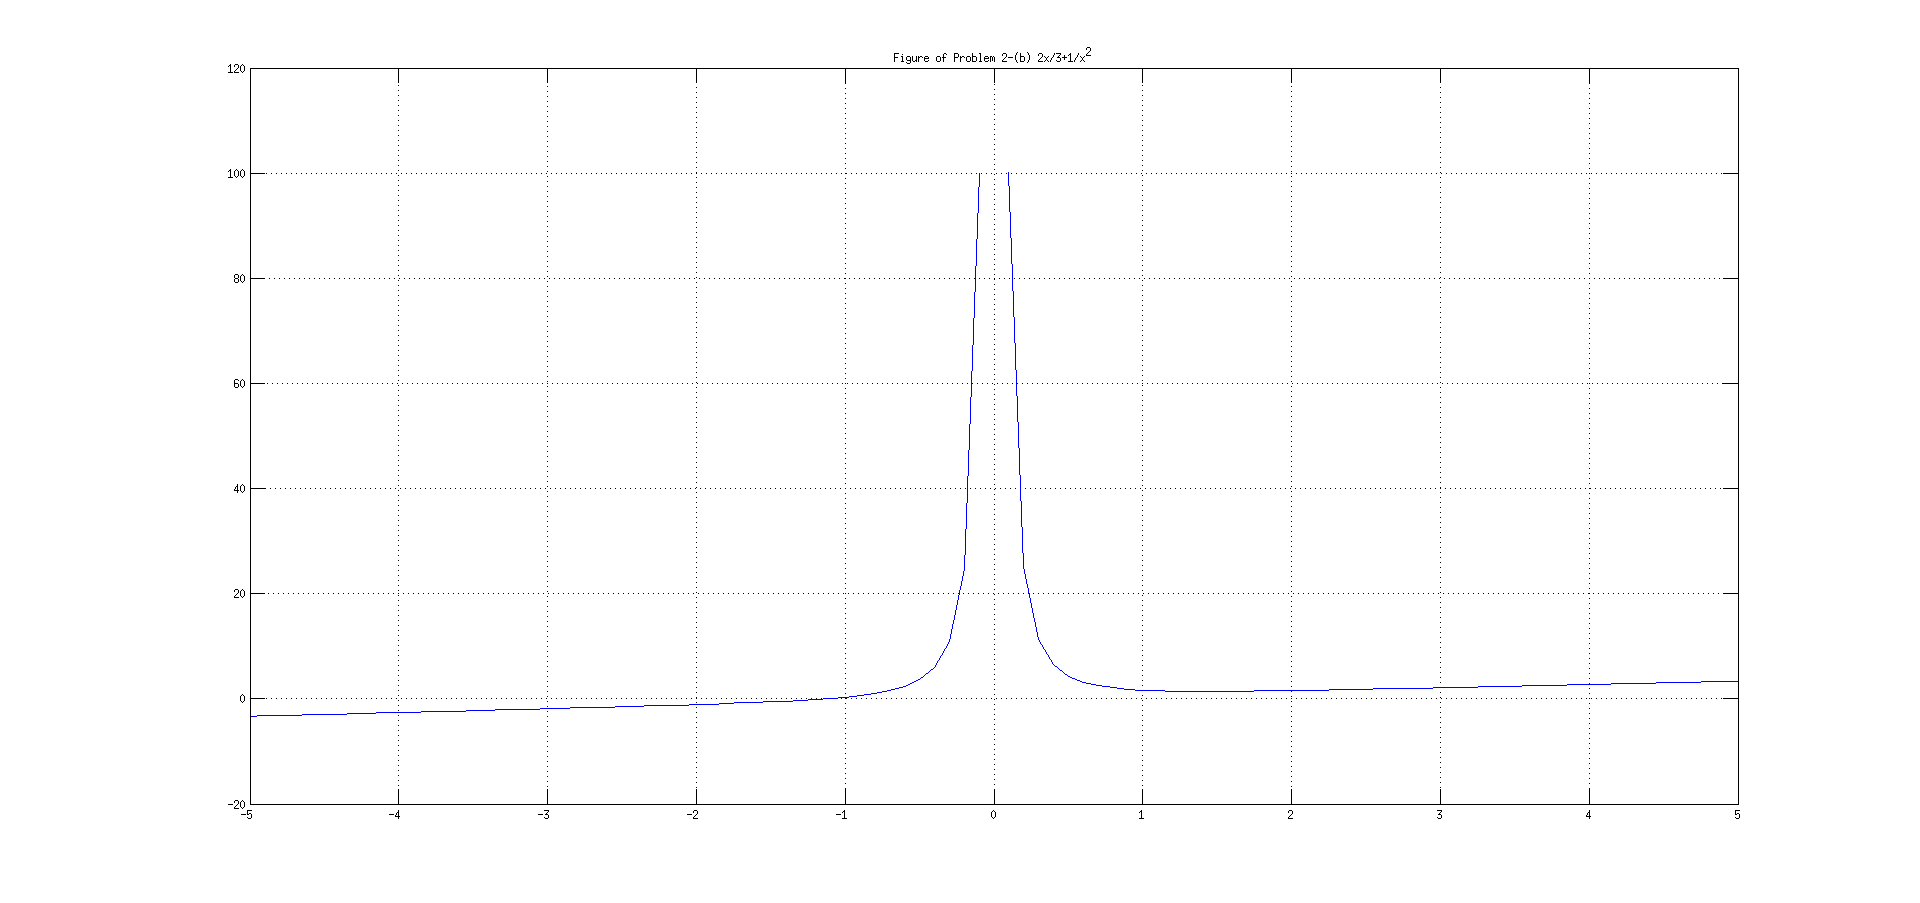
\includegraphics[width=1\textwidth]{2-b.png}
		\caption{Problem 2-(b), $-2x/3+1/x^2$ }
		\end{center}
	\end{figure}
	\qquad \quad We can know $f(x)$ have root. Using Fixed Point Method, \\
	\begin{figure}[!h]
		\centering
		\begin{center}
		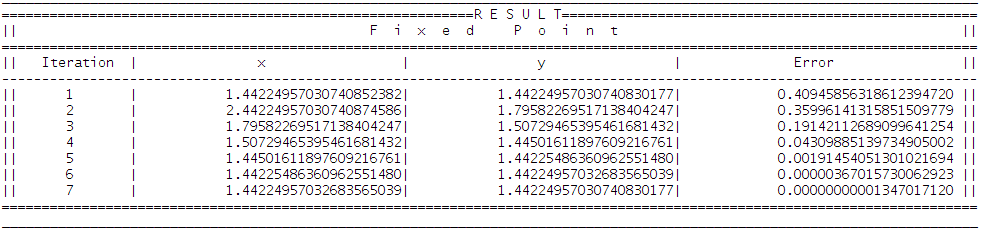
\includegraphics[width=0.9\textwidth]{2-rb.png}
		\caption{Problem 2-(b), Result}
		\end{center}
	\end{figure}
	\qquad \quad We choose initial condition. $x_0=3^{\frac{1}{3}}+\epsilon$ and relative error boundary less than $\epsilon$.\\
	\qquad \quad We can know this function is convergence using fixed point method.Therefore, convergence rate is\\
	\;\;\;
	\qquad \qquad \qquad \qquad\quad$f(x_n)-(\alpha+\epsilon)=r(x_n-(\alpha+\epsilon)) \rightarrow \, x_{n+1}-(\alpha+\epsilon)=r(x_n-(\alpha+\epsilon))$\\
	\qquad\qquad\qquad\qquad\qquad\qquad\qquad\qquad\qquad\qquad\qquad\qquad$\rightarrow \, r=\frac{x_{n+1}-(\alpha+\epsilon)}{x_n-(\alpha+\epsilon)}$\\
	\qquad\qquad\qquad\qquad\qquad\qquad\qquad\qquad\qquad\qquad\qquad\qquad$\rightarrow \, r=g(\alpha) \thickapprox \frac{x_{n+1}-\alpha+\epsilon}{x_n-\alpha+\epsilon}$    (Using I.V.T)\\
	\qquad\qquad\qquad\qquad\qquad\qquad\qquad\qquad\qquad\qquad\qquad\qquad$\rightarrow \, r=-\frac{1}{3}$.\\
	\;\;\;
	\qquad \quad Since $f'(x)=\frac{2}{3}-3x^{-3}$. Therefore, convergence rate is $-\frac{1}{3}$.\\
	\;\;\;\;\newpage
	\quad\,\textbf{(c)} $x_{n+1}=12/(1+x_n),\quad \alpha=3$\\
	\;\;\;
	\qquad \quad \textbf{(Solution.)} \\
	\qquad \quad Similary, Before using Fixed Point Method, Looking at Graph of $f(x)=12/(1+x_n)$\\
	\begin{figure}[!h]
		\centering
		\begin{center}
		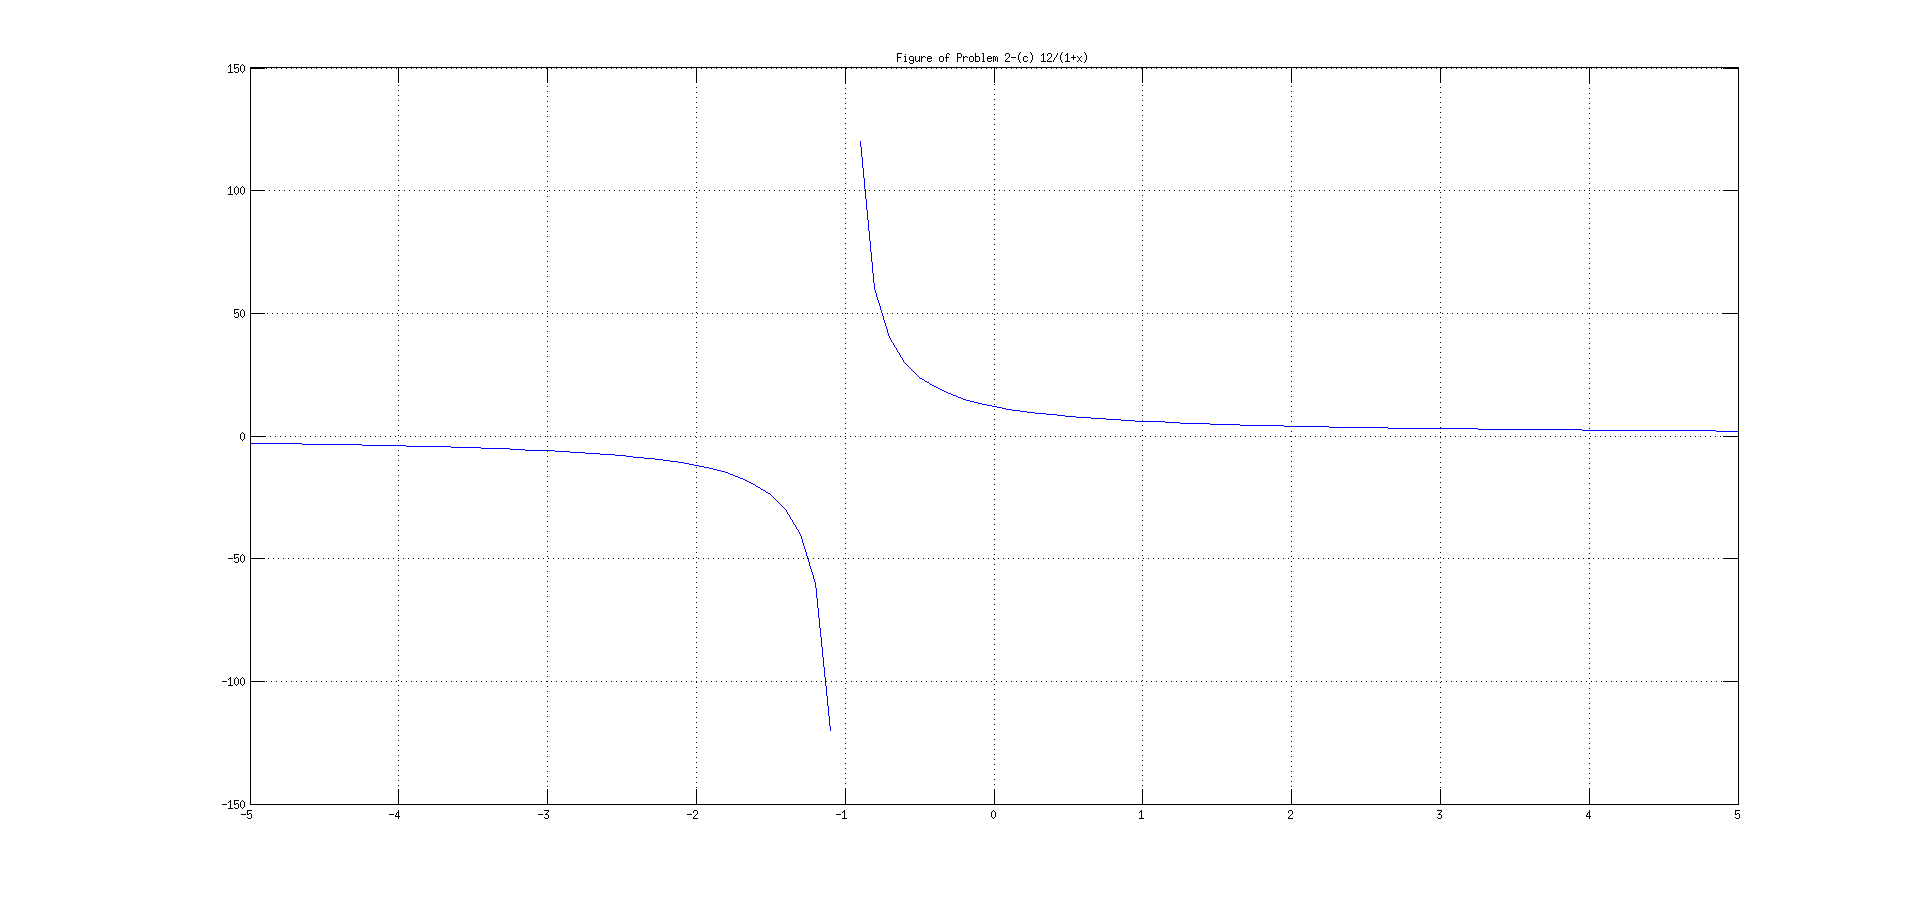
\includegraphics[width=1\textwidth]{2-c.png}
		\caption{Problem 2-(c), $12/(1+x_n)$ }
		\end{center}
	\end{figure}
	\qquad \quad We can know $f(x)$don't have root. Using Fixed Point Method, \\
	\begin{figure}[!h]
		\centering
		\begin{center}
		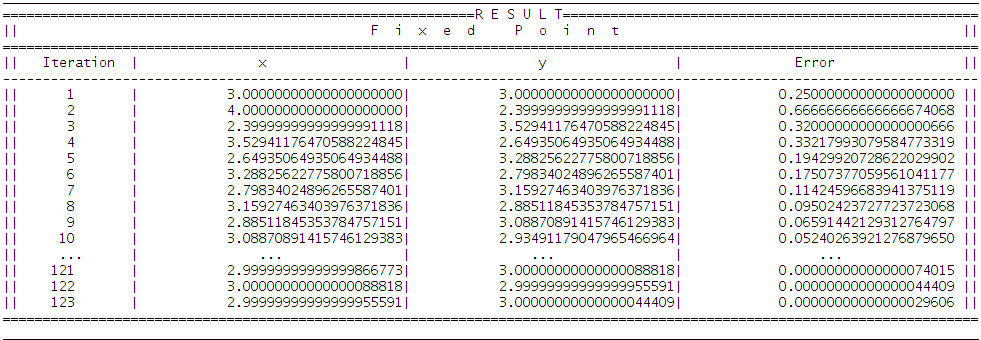
\includegraphics[width=0.9\textwidth]{2-rc.png}
		\caption{Problem 2-(c), Result}
		\end{center}
	\end{figure}
	\qquad \quad We choose initial condition. $x_0=3+\epsilon$ and relative error boundary less than $\epsilon$.\\
	\qquad \quad We can know this function is convergence using fixed point method.Therefore, convergence rate is\\
	\;\;\;
	\qquad \qquad \qquad \qquad\quad$f(x_n)-(\alpha+\epsilon)=r(x_n-(\alpha+\epsilon)) \rightarrow \, x_{n+1}-(\alpha+\epsilon)=r(x_n-(\alpha+\epsilon))$\\
	\qquad\qquad\qquad\qquad\qquad\qquad\qquad\qquad\qquad\qquad\qquad\qquad$\rightarrow \, r=-\frac{3}{4}$.\\
	\;\;\;
	\qquad \quad Since $f'(x)=-\frac{12}{(1+x)^2}$. Therefore, convergence rate is $-\frac{3}{4}$.\\
	\;\;\;\;
	\qquad \quad \textbf{- Comment}\\
	\qquad \qquad We investigated the convergence. We calculated convergence rate of (b) and (c), When the other\\
	\qquad \qquad problem (a) compute convergence rate $r=3$.\\
	\qquad \qquad We can know $\vert r \vert <1$ is convergence, $\vert r \vert >1$ is divergence. And we can know slow convergence and\\
	\qquad \qquad divergence when r is closer 1. Above all the reason is \\
	\qquad \qquad \qquad \qquad\qquad\qquad\qquad\qquad$x_{n+1}-\alpha=r(x_n-\alpha) \rightarrow \, E_{n+1}=rE_n$.\\
	\qquad \qquad Therefore, If $r$ increase, Error is more and more increased by $r$.
	\newpage
	\textbf{3.} Consider the system\\
	\;\;\;
	\qquad \qquad \qquad \qquad\qquad\qquad\qquad\qquad\qquad $x=\frac{0.5}{1+(x+y)^2},\quad y=\frac{0.5}{1+(x-y)^2}$\\
	\;\;\;
	\quad\, Find a bouded region $D$ for which the hypotheses of Theorem in page 10 of NA lecture note $\#1$ are \\
	\quad\: satisfied.\\
	\;\;\;
	\quad\: \textbf{(Solution.)} \\
	\quad\: The hypotheses of Theorem in page 10 of NA lecture note\\
	\;\;\;
	\qquad\qquad\qquad\qquad $g(D)\subset D,\quad \lambda \equiv max_{x \in D} \Vert G(x) \Vert_{\infty} \rightarrow \exists !$solution and convergenc in $D$ to $\alpha$.\\
	\;\;\;
	\quad\: We can calculate Boundary condition, substituting $(x+y)^2$ to $T$.\\
	\quad\: Boundary of$x=\frac{0.5}{1+T^2}$ is\\
	\qquad\qquad\qquad\qquad\qquad\qquad\qquad\qquad\qquad $\rightarrow T^2 \geq 0$\\
	\qquad\qquad\qquad\qquad\qquad\qquad\qquad\qquad\qquad $\rightarrow 1+T^2 \geq 1$\\
	\qquad\qquad\qquad\qquad\qquad\qquad\qquad\qquad\qquad $\rightarrow \frac{1}{1+T^2} \leq 1$\\
	\qquad\qquad\qquad\qquad\qquad\qquad\qquad\qquad\qquad $\rightarrow \frac{0.5}{1+T^2} \leq 0.5$\\
	\;\;\;
	\quad\: Therefore, $x \leq 0.5$, we can compute $y$ using simlar manner. $y \leq 0.5$.\\
	\quad\: For recheck, Using Matlab, (Initical condition $x_0=0.5,\:y_0=0.5$)\\
	\begin{figure}[!h]
		\centering
		\begin{center}
		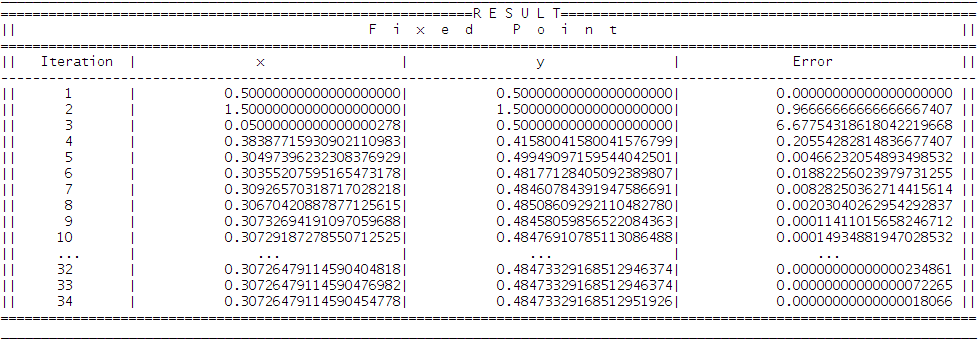
\includegraphics[width=0.9\textwidth]{3-r.png}
		\caption{Problem 3, Result}
		\end{center}
	\end{figure}
	\quad\: Therefore, we can know that calculated boudary $D=\{(x,y)\vert x\in(0,0.5],\:y\in(0,0.5]\}$.\\
	\quad\: Once again, we are running iteration 1000 using random function to select initial condition.\\
	\begin{figure}[!h]
		\centering
		\begin{center}
		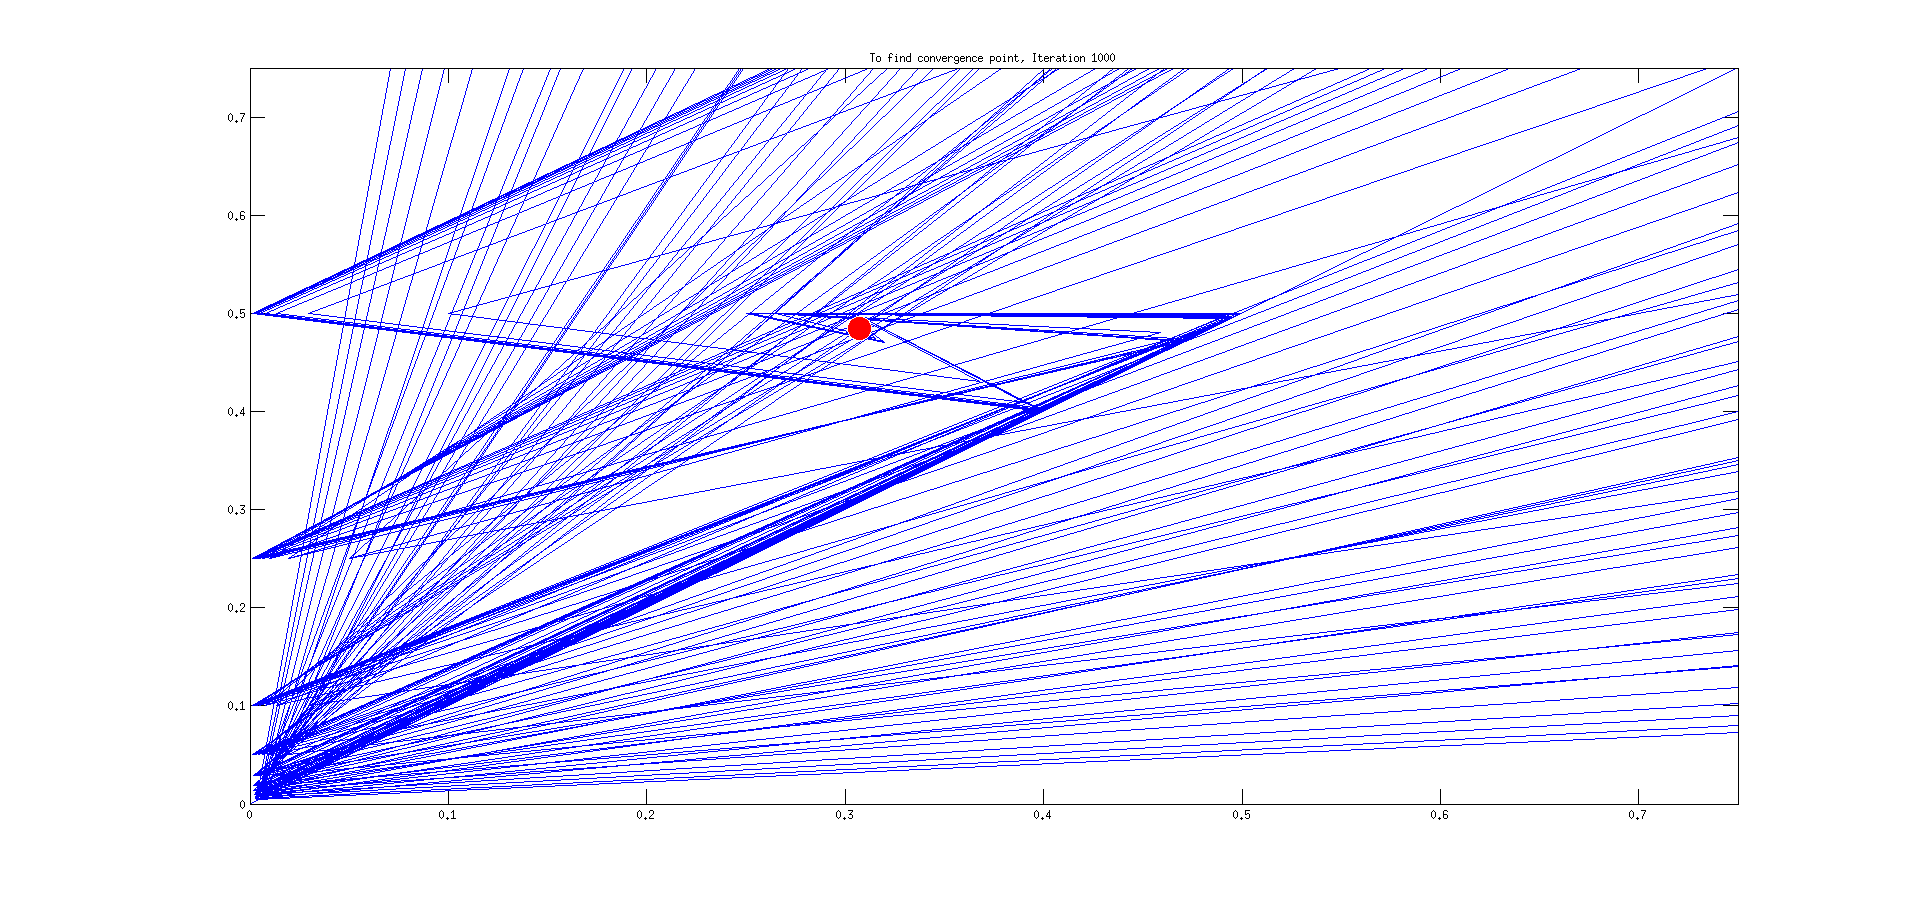
\includegraphics[width=0.8\textwidth]{3.png}
		\caption{Problem 3, Random initial condition, iteration 1000 }
		\end{center}
	\end{figure}
	\quad\: Therefore, we know this function is started at some initial point. Convergence point is about $(0.30,0.48)$.
	\newpage
	\textbf{4.} Consider\\
	\;\;\;
	\qquad \qquad \qquad \qquad\qquad\qquad\qquad\qquad\qquad $f(x)=\frac{1}{1+x^2},\quad -5 \leq x \leq 5$\\
	\;\;\;
	\quad\, Use Lagrange's formula and Newton's divided difference formula to construct $p_6,p_8,p_{10}$ and $p_{16}$ \\
	\quad\, interpolation polynomials in uniformly divided interval.\\
	\;\;\;
	\quad\: \textbf{(Solution.)} \\
	\quad\: To solve this problem, We can know disadvantage of Lagrange and Newton interpolation.\\
	\quad\: We already knew that Newton is computing better than Langrange. Priority, comparing Original with \\
	\quad\: Numerical function,\\
	\begin{figure}[!h]
		\centering
		\begin{center}
		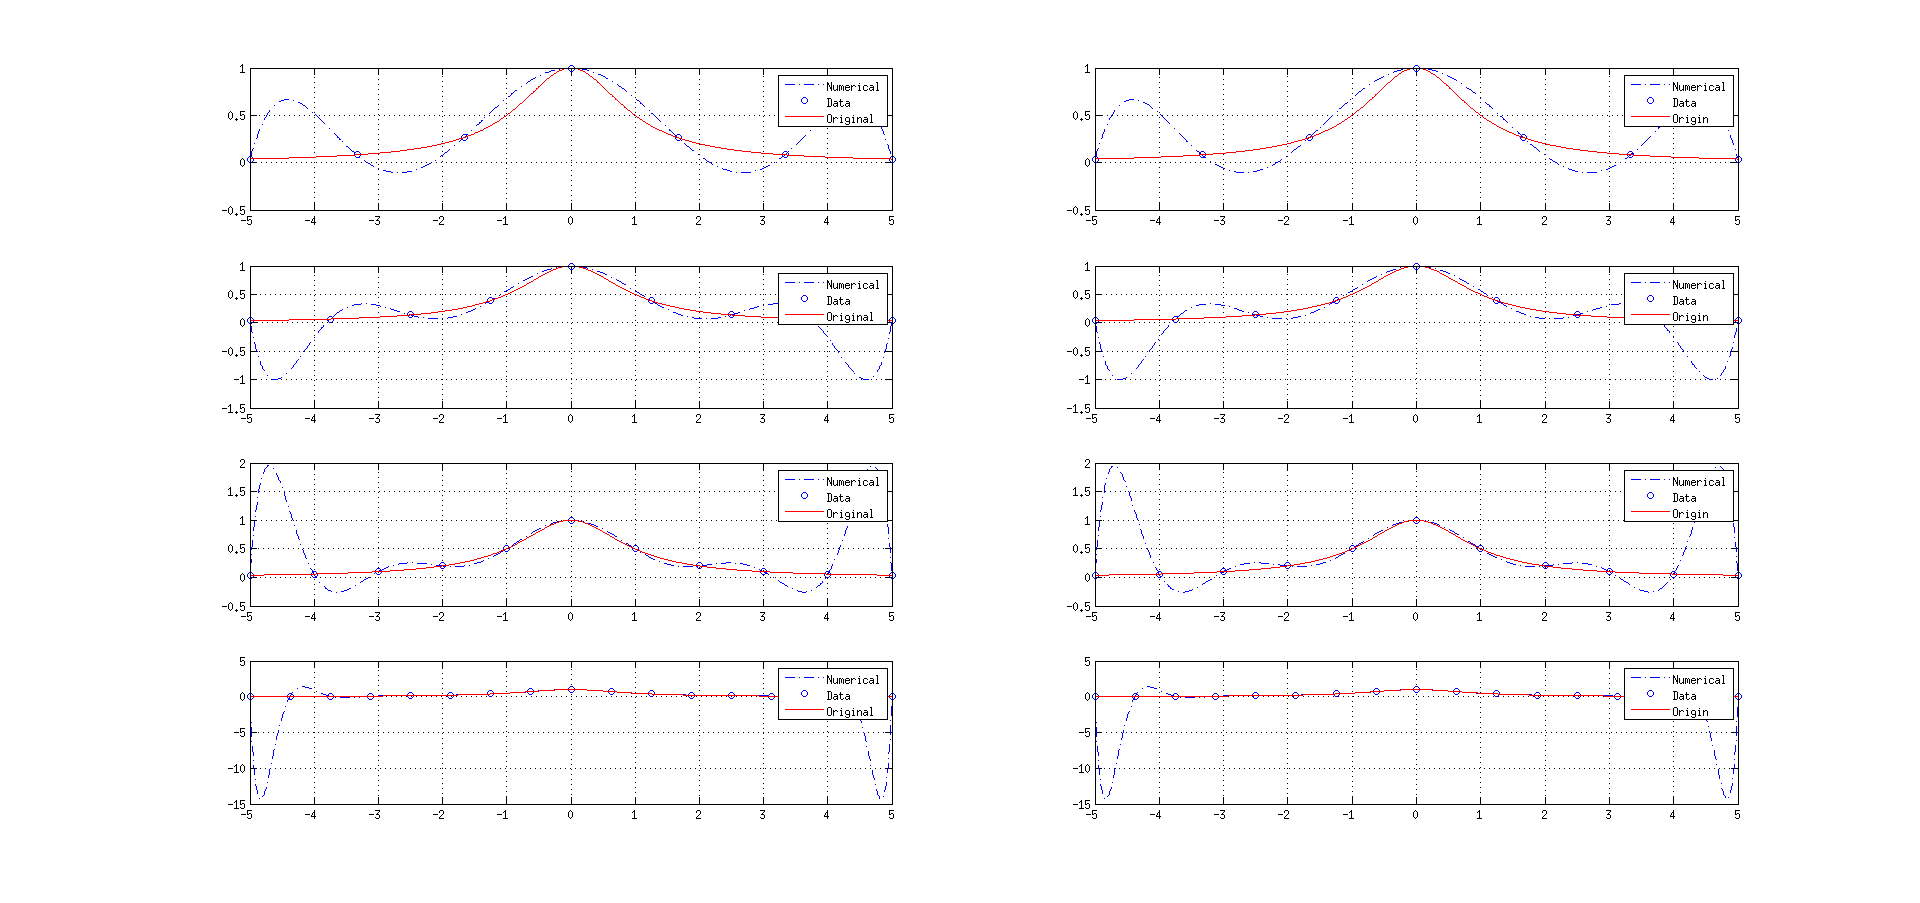
\includegraphics[width=1\textwidth]{4.png}
		\caption{Problem 4, Left figure is f(x) vs Lagrange.Right figure is f(x) vs Newton }
		\end{center}
	\end{figure}
	\quad\: Two method is similar result. Results show that each degree.\\
	\begin{figure}[!h]
		\centering
		\begin{center}
		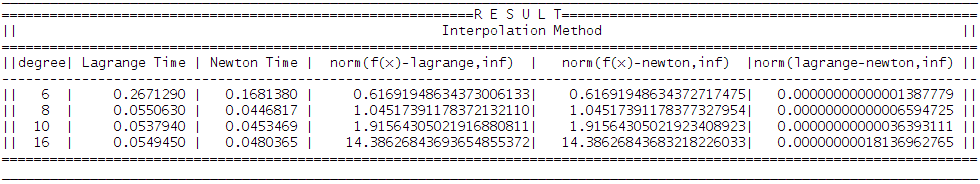
\includegraphics[width=0.9\textwidth]{4-r.png}
		\caption{Problem 4, Result}
		\end{center}
	\end{figure}
	\quad\: You can see Newton time is shorter than Lagrange. And Lagrange is similar to Newton.\\
	\quad\: But two interpolation have ocillation at boundary. Therefore, we need other method to minimize ocillation.\\
	\quad\: Other method mean piecewise interporation using some a condition. Next problem (5) is Spline which is\\
	\quad\: piecewise interporation.\\
	\newpage
	\textbf{5.} Consider the same function $f(x)$ given in "problem4" and consider\\
	\;\;\;
	\qquad \qquad \qquad \qquad\qquad\qquad\qquad $x_k=-5+k(10/16),\quad y_k=f(x_k),$ for $k=0,1,...,16$\\
	\;\;\;
	\quad\, Construct cubic sspline interpolation and compare the result with the results when $p_{16}$ polynomial was \\
	\quad\, used in "problem4"-interpolation.\\
	\;\;\;
	\quad\: \textbf{(Solution.)} \\
	\quad\: Cubic Spline is piecewise interpolation. Therefore, we can expect more and more exact solution.\\
	\quad\: Prior to the description, Cubic Spline end-conditions are Natural, Complete and Not-A-Knot. Each \\
	\quad\: condition is simila to boundary condition.\\
	\quad\: In some cases, We can select end-condition. This problem compare Problem (4) with 3 case of Cubic \\
	\quad\: Spline. First, 3 condition of Cubic Spline are\\
	\begin{figure}[!h]
		\centering
		\begin{center}
		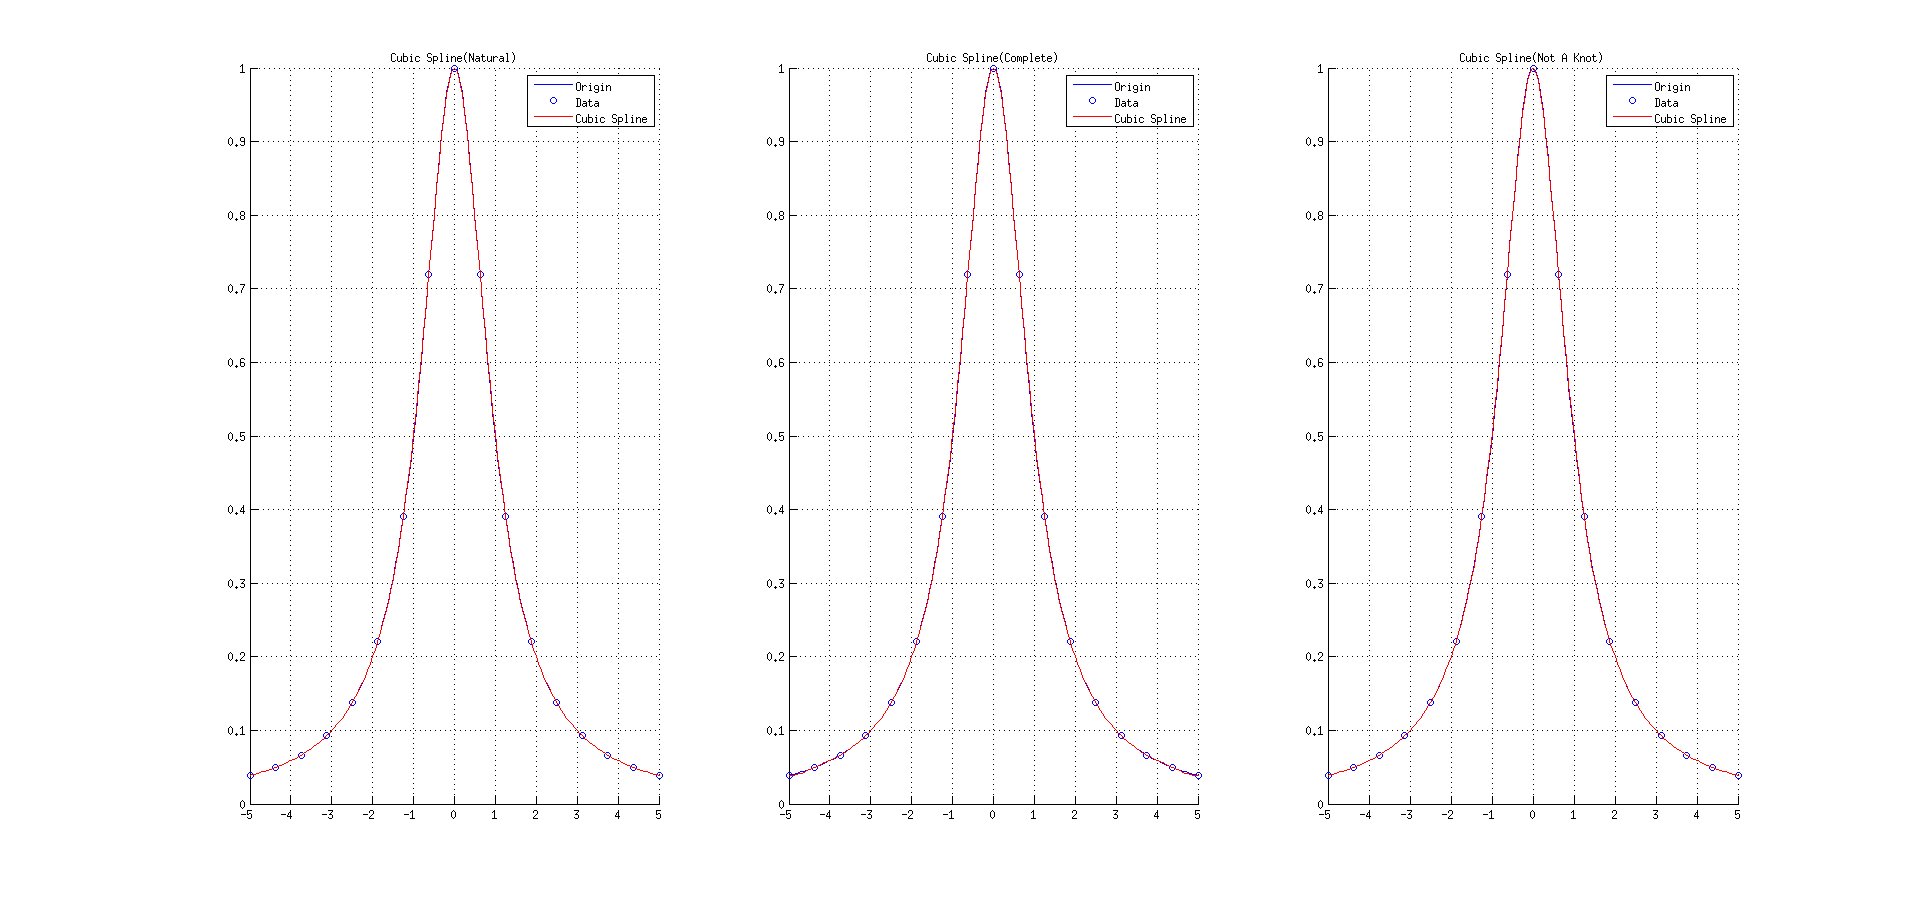
\includegraphics[width=1\textwidth]{5.png}
		\caption{Problem 5, Natural Condition vs. Complete Condition vs. Not-A-Knot Condition. }
		\end{center}
	\end{figure}
	\quad\: We can know that this problem is not good using Complete Condition. Because boudary have a few\\ 		\quad\: ocillation. But Cubic Spline have result better than problem (4). Examined error is\\
	\begin{figure}[!h]
		\centering
		\begin{center}
		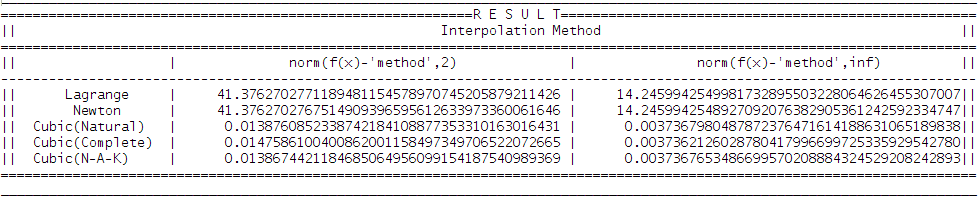
\includegraphics[width=0.9\textwidth]{5-r.png}
		\caption{Problem 5, Result}
		\end{center}
	\end{figure}
	\quad\: Therefore, We can exactly know that Cubic Spline of piecewise interporation is better than Lagrange and \\
	\quad\: Newton interpolation.  
  	\end{flushleft}
\end{document}